\section{Termination, Soundness and Completeness}\label{sec:correct}


We show the procedure terminates in deterministic exponential time (\S\ref{ss:term}), is sound
for all of TCTL, and is complete over the non-punctual fragment (\S\ref{ss:sound}). Throughout,
$\varphi$ is the input formula, $n=|\FL(\varphi)|$, and $M$ the largest constant in its
intervals.
\subsection{Termination and Complexity}\label{ss:term}

To prove termination and \textsc{ExpTime}-completeness, we proceed in two steps. First, we bound the number of distinct nodes the procedure can generate, and then we show that the marking can be computed within that budget.

%First, we prove the procedure terminates and it is \textsc{ExpTime}-complete. To do so, we first bound the number of distinct nodes the procedure can generate.
\begin{lemma}\label{lem:finiteness}
The number of distinct nodes the procedure can generate is bounded above by $2^{O(n)}\cdot M^{O(n^2)}$.
\end{lemma}

\begin{proof}
The propositional components $\Gamma,\Ctx$ range over subsets of $\FL(\varphi)$, hence
$2^{O(n)}$ choices each; the clock map $\obligations$ over $2^{O(n)}$ assignments and $\Deadline$ over $2^{O(n)}$ choices. The cover rule allocates one
formula-clock per timed subformula, bounded by $O(n)$. A canonical $\cong_M$-zone over $K$
clocks is a $(K{+}1)^2$ DBM whose finite entries lie in $\{-M,\dots,M\}\times\{<,\le\}$,
giving $M^{O(K^2)}\le M^{O(n^2)}$ distinct zones. Multiplying the components yields $2^{O(n)}\cdot M^{O(n^2)}$.
\end{proof}



Now we can prove the main result of this section.



\begin{theorem}\label{thm:complexity}
Satisfiability of non-punctual TCTL is \textsc{ExpTime}-complete, and the tableau
decides it in time $2^{\mathrm{poly}(n)}$.
\end{theorem}
\begin{proof}
Let $m=2^{O(n)}\cdot M^{O(n^2)}$ be the node bound of Lemma~\ref{lem:finiteness}; since the
encoding of $M$ occupies at most $n$ input symbols, $\log m=O(n)+O(n^2)\log M=\mathrm{poly}(n)$.
Nodes are drawn from a set of size $m$, so the memoised AND--OR graph has at most $m^2$ edges;
by the pigeonhole principle every infinite branch repeats a node, where the loop rule adds a
back-edge or closes, and the construction halts after at most $m$ expansions. Memoisation ensures each node is expanded at most once, avoiding the doubly exponential
blow-up of the naive ancestor-only unfolding.
%
%Memoisation is
%essential rather than an optimisation: with ancestor-only loop detection the same graph unfolds
%to a doubly-exponential tree.

The satisfaction sets are computable within this budget. Each
$\Sat_{\Ctx}(\mu)$ is a least ($\mathbf{U}$) or greatest ($\mathbf{R}$) fixpoint of a monotone map on unions of $\cong_M$-zones, which are at most $M^{O(n^2)}$ in number, thus finite, so by Knaster--Tarski the
fixpoint exists and monotone iteration reaches it in as many steps, each a polynomial number of
DBM operations, with a factor $O(n)$ over $\FL(\varphi)$.


A successful marking is then found by the standard elimination procedure for
AND--OR tableaux~\cite{Clarke99,tableau_ctl}: repeatedly delete every closed node,
every OR-node whose children are all deleted, every AND-node with a deleted
child, every node from which no surviving path reaches a time-progressing loop,
and every node from which no surviving path takes the \ruleref{Ustop} branch of
an until pursuit active there. The first three tests are local; the last two are
reachability queries over the surviving subgraph, each decidable in time
polynomial in $m$, and it is sound to recompute them each round because deletion
only ever removes paths, never creates them. The two queries enforce conditions
(ii) and (i) of \S\ref{ss:loop} respectively. Each round deletes at least one
node, so at most $m$ rounds suffice, and $\varphi$ is satisfiable iff the root
survives. The procedure therefore runs in $2^{\mathrm{poly}(n)}$.

Hardness is inherited: fixing every interval to $[0,\infty)$ the procedure decides CTL
satisfiability, which is \textsc{ExpTime}-hard~\cite{Clarke99}.


%
%It remains to decide existence of a successful marking. A marking retains all AND-children, so
%goodness of every infinite path is a universal condition over the AND-branching: an AND-fork into one good and one bad cycle is rejected. Existence is therefore
%the winning condition of a two-player game on the finite graph --- the proponent resolving the
%OR-choices, the opponent the AND-branches and the path --- won by the proponent iff every play
%is an accepting lasso, every eventuality fulfilled and time-progressing by
%Lemma~\ref{lem:nonzeno}. This is a Streett condition with $k=O(n)$ pairs, one per eventuality
%and one per delay-bounding clock, solved by the standard nested-fixpoint algorithm in
%$m^{O(k)}=2^{O(k\log m)}$, singly exponential in $n$.
%
%Hardness is inherited: fixing every interval to $[0,\infty)$ the procedure decides CTL
%satisfiability, which is \textsc{ExpTime}-hard~\cite{Clarke99}.
\end{proof}










\subsection{Soundness and Completeness}\label{ss:sound}

We now prove the procedure is sound, i.e., that if the tableau succeeds on $\varphi$, then $\varphi$ is \SAT, and complete, i.e., that if $\varphi$ is \SAT, then the tableau succeeds on $\varphi$. These results are supported by the following lemmas. 

%
%By finiteness a successful marking $\mathcal{M}$ is a finite AND--OR structure whose infinite paths are
%lassos $\pi_{\mathsf{pref}}\cdot\pi_{\mathsf{loop}}^\omega$ with an accepting loop~\cite{Clarke99}. From
%$\mathcal{M}$ we build a witness TTS $\mathcal{T}$, then verify it by induction. Three lemmas support the
%construction: one makes the zones realisable as delays, one reconciles the discrete induction with the dense
%semantics, and one guarantees time divergence.
%

\begin{lemma}\label{lem:feasible}
Let $N_0,\dots,N_k$ be a finite path of $\mathcal{M}$ with non-empty zones. For every
$\nu_k\in Z_k$ there are $\nu_0\in Z_0,\dots,\nu_{k-1}\in Z_{k-1}$ and positive delays
realising every step.
\end{lemma}
\begin{proof}
Each operation used along a path (intersection and guards,
reset, time-successor and
$\cong_M$-canonicalisation) admits back-propagation, non-empty
precisely because the successor valuation lies in its image~\cite{Bouyer05TimedAutomata}; threading
backward from $\nu_k$ gives the assignment.
\end{proof}

%\begin{lemma}[Feasibility]\label{lem:feasible}
%Along any finite path of $\mathcal{M}$ whose nodes carry non-empty zones, there is a consistent assignment of
%clock valuations and delays realising every time-elapse and reset step.
%\end{lemma}
%\begin{proof}
%The zone operations the path uses -- intersection, single-clock guard $x\in\kI$, reset $Z[R{:=}0]$,
%time-successor $\uparrow Z$, and $\cong_M$-canonicalisation -- each preserve non-emptiness and, given a
%representative of the successor zone, admit a compatible representative of the predecessor zone (the standard
%DBM back-propagation~\cite{AlurDill1994,Bouyer05TimedAutomata}). Threading representatives from the end of the
%path backward yields valuations and positive delays consistent with every step.
%\end{proof}
%
\begin{lemma}\label{lem:stability}
Along a delay step $(s,\nu)\xrightarrow{t}(s,\nu+t)$ that crosses no integer hyperplane $x=b$ ($b\le M$), the
truth of every subformula of $\varphi$ is constant over the relatively-open segment $(s,\nu+t')$,
$t'\in(0,t)$.
\end{lemma}

\begin{proof}
Crossing no hyperplane $x=b$ with $b\le M$, no clock crosses an integer at or below $M$, so
no integer part changes and no fractional ordering wraps; clocks already above $M$ are
identified by extrapolation and their exact values are immaterial. All $(s,\nu+t')$
therefore lie in one clock region, and TCTL truth is constant on a
region~\cite{AlurCourcoubetisDill1990,Bouyer05TimedAutomata}.
\end{proof}
\noindent
The endpoints, where a clock sits exactly on a hyperplane, are nodes of their own by the
integer split of \ruleref{Delay}: a guard $x_\mu\in\kI$ is then tested against the zone
$x_\mu=b$, and whether it holds there is decided by the strictness flag of $\kI$'s endpoint.

%\begin{proof}
%Crossing no such hyperplane, no clock changes integer part below $M$ and no fractional ordering wraps, so all
%$(s,\nu+t')$ lie in one clock region; TCTL truth is constant on a region (the region
%theorem~\cite{AlurCourcoubetisDill1990,Bouyer05TimedAutomata}). The integer-split of successor generation
%makes the segment endpoints, where a clock may sit on a hyperplane, into nodes, handled by the strictness
%flags of the interval bounds. Diagonal-freeness and integer endpoints suffice; non-punctuality is not needed
%here.
%\end{proof}

\begin{lemma}\label{lem:nonzeno}
A candidate loop $N_i \equiv N_j$ has a non-Zeno unfolding iff it is {time-progressing}: it admits positive total elapsed time and every clock is either reset on the segment or extrapolated above $M$, hence unbounded.
When it is, a run exists in which every iteration elapses the same positive amount%, i.e. $\exists \delta >0$ such that every iteration elapses time $\delta$
.
\end{lemma}
\begin{proof}
($\Rightarrow$) By contraposition, suppose the loop is not time-progressing.  Either it elapses no time, in which case infinitely many traversals take zero
time in total, or some clock $x$ is neither reset on the segment nor extrapolated above $M$,
and so retains a finite bound $x\le c$ with $c\le M$ in the zones of the loop. In the second
case $x$ is unreset, so it increases by exactly the delay elapsed on each traversal, and the
bound is enforced at every node; the delays of all iterations together therefore sum to at most
$c-\nu(x)$, and infinitely many delays with a finite sum converge. Either way the unfolding is
Zeno.

($\Leftarrow$) Suppose the loop is time-progressing. Lemma~\ref{lem:feasible} yields a
traversal over the loop with some $\delta>0$. Since $N_i\equiv N_j$, no rule distinguishes
the two visits and the traversal is repeated; no budget depletes either, each clock being
reset on the segment or extrapolated above $M$, leaving it unbounded. 
Hence $\delta$ recurs at every iteration, yielding the last claim and $\sum_k t_k\ge\sum_k\delta=\infty$.
\end{proof}




\begin{lemma}\label{lem:sat}
Let $\mu$ be demanded at $N$ under $\Ctx$, $\nu\in Z_N$, and let $\mathcal{T}$ be the TTS
read off a successful marking containing $N$, with $s_N$ the location of $N$. Moreover, let $\mathcal{T}'$ be any TTS with configuration $(s,\nu)$ satisfying $\Ctx$. Then
\[
  (i)\ \nu\in\Sat_{\Ctx}(\mu)\ \Longrightarrow\ \mathcal{T},(s_N,\nu)\models\mu,
  \qquad
  (ii)\ \mathcal{T}',(s,\nu)\models\mu\ \Longrightarrow\ \nu\in\Sat_{\Ctx}(\mu)
\]
\end{lemma}



\begin{proof}

By Lemma~\ref{lem:stability}, since no delay step crosses a hyperplane, the truth of every subformula is constant along the open segment between consecutive nodes, letting us argue at nodes throughout. 


Write $\Sat_{\Ctx}(\mu)^{k}$ for the valuations obtained after $k$ unfoldings: for an until, those reaching a
base child within $k$ steps, so the $\Sat_{\Ctx}(\mu)^{k}$ grow from $\emptyset$; for a release, those violating
the obligation at no step among the first $k$, so the $\Sat_{\Ctx}(\mu)^{k}$ shrink from the universal zone. By
construction, $\nu\in\Sat_{\Ctx}(\mu)$ means $\nu\in \Sat_{\Ctx}(\mu)^{k}$ for some $k$ in the first case and
for every $k$ in the second, and both sequences stabilise after finitely many steps.

\textit{\lemitem{lem:sat}{i}} By construction, the runs of $\mathcal{T}$ from $(s_N,\nu)$ correspond to the pursuit paths from $N$,
since the discrete edges of $\mathcal{T}$ are the pursuits' $\EX/\AX$-successors (\ruleref{Cov} contributes none).
\noindent
For an until, we proceed by induction on the least $k$ with $\nu\in \Sat_{\Ctx}(\mu)^{k}$. If $k=1$ then $\nu$ lies in a base
zone, so the $\ruleref{Ustop}$ branch applies: $\psi$ holds at $(s_N,\nu)$ with $x_\mu\in\kI$, and
\eqref{eq:sat_u} is met at the current position. If $k>1$ then $\nu$ matches a $\ruleref{Ugo}$
child, so $\varphi$ holds at $(s_N,\nu)$ and the deferred successors lie in $\Sat_{\Ctx}(\mu)^{k-1}$; by
induction $\mu$ holds at each, and prepending the current position gives a run satisfying
\eqref{eq:sat_u}. The quantifier follows from the child: for $\mathrm{Q}=\mathrm{E}$ one
successor is demanded and the run through it witnesses $\exists\rho$; for
$\mathrm{Q}=\mathrm{A}$ all are, and every run of $\mathcal{T}$ begins with one of them, giving
$\forall\rho$. The deadline in $\Inv(N)$ stops a universal run idling past the window.

\noindent
For a release, the hypothesis gives $\nu\in \Sat_{\Ctx}(\mu)^{k}$ for every $k$. Fix a position $\pi=(i,\delta)$ of a run from $(s_N,\nu)$. It is reached after $i$ discrete steps, so taking $k=i+1$ the hypothesis gives that the obligation is not violated at $\pi$:
either $\psi$ holds there or an earlier $\varphi$ released it. As $\pi$ was arbitrary this is \eqref{eq:sat_r}, for one run when
$\mathrm{Q}=\mathrm{E}$ and for all when $\mathrm{Q}=\mathrm{A}$.

\textit{\lemitem{lem:sat}{ii}} Here $\mathcal{T}'$ is arbitrary, so we read a path off a run rather than
building one. A run satisfying \eqref{eq:sat_u} reaches $\psi$ at a position $(i,\delta)$ with
$i$ finite, and selecting at each step the branch the run takes gives a path into a base child
in $i$ steps, so $\nu\in \Sat_{\Ctx}(\mu)^{i}$. For $\mathrm{Q}=\mathrm{E}$ one such run suffices; for
$\mathrm{Q}=\mathrm{A}$, every run gives one such path, and, since the pursuit graph is finitely branching (each rule has finitely many children and Lemma~\ref{lem:finiteness}), by K\"onig's lemma a single $k$ bounds them all, so $\nu\in \Sat_{\Ctx}(\mu)^{k}$. For a release we show $\nu\in \Sat_{\Ctx}(\mu)^{k}$ by induction
on $k$: the obligation is met at the current position, since \eqref{eq:sat_r} holds along the
runs of $\mathcal{T}'$, and the successors inherit the hypothesis, so $\nu$ survives every
stage.

\end{proof}


%
%
%\begin{lemma}\label{lem:sat}
%Let $\mu$ be demanded at a node $N$ under context $\Ctx$, and let $\nu\in Z_N$.
%\begin{enumerate}
%\item[(i)] If $\nu\in\Sat_{\Ctx}(\mu)$ then $\mathcal{T},(s_N,\nu)\models\mu$, where
%  $\mathcal{T}$ is the TTS read off the pursuit branches of a successful marking containing $N$
%  and $s_N$ the location it assigns to $N$.
%\item[(ii)] If $\mathcal{T}',(s,\nu)\models\mu$ for any TTS $\mathcal{T}'$ and configuration
%  $(s,\nu)$ at which $\Ctx$ holds, then $\nu\in\Sat_{\Ctx}(\mu)$.
%\end{enumerate}
%\end{lemma}
%\begin{proof}
%
%%By construction, $\Sat_{\Ctx}(\mu)$ tracks the path quantifier of \eqref{eq:until}--\eqref{eq:release}
%%
%%
%%A valuation lies in $\Sat_{\Ctx}(\mu)$ if it lies in a base child of \ruleref{Uunf} or \ruleref{Rsplit}, or in
%%a recursive child whose deferred successors lie in $\Sat_{\Ctx}(\mu)$, one successor when
%%$\mathrm{Q}=\mathrm{E}$ and all of them when $\mathrm{Q}=\mathrm{A}$. This is
%%\eqref{eq:until}--\eqref{eq:release} read one step at a time, the path quantifier tracked by
%%where the residual travels, $\EX\mu^\bullet$ into $\Gamma$ and $\AX\mu^\bullet$ into $\Ctx$. By
%%construction, $\Sat_{\Ctx}(\mu)$ is the least fixpoint of $F$ for an until and the greatest
%%for a release, and Lemma~\ref{lem:stability} lifts each step from the nodes to the dense
%%positions between them.
%%
%%
%%$\Sat_{\Ctx}(\mu)$ is a fixpoint of the pursuit unfolding, and that unfolding mirrors the
%%semantic clause one step at a time, relative to $\Ctx$. The quantifiers of \eqref{eq:sat_u}--\eqref{eq:sat_r} are matched by the $\EX/\AX$-successors of the pursuit and the operator fixes which fixpoint of that equation is
%%taken: least for until, so membership means reaching a stop in finitely many steps; greatest
%%for release, so membership means never violating the obligation. Using Lemma~\ref{lem:stability}, each step is lifted from the nodes to the dense positions between them. Accordingly:
%%
%By construction, a valuation enters $\Sat_{\Ctx}(\mu)$ through one child of \ruleref{Uunf} or
%\ruleref{Rsplit} at each stage of the iteration, so its membership is witnessed by a pursuit
%path. Lemma~\ref{lem:stability} extends that path between consecutive nodes: no delay step
%crosses a hyperplane, so each open segment lies in one region and agrees with the nodes
%bounding it.
%
%\textit{(i)} The runs of $\mathcal{T}$ from $(s_N,\nu)$ are the pursuit paths from $N$:
%the discrete edges of $\mathcal{T}$ are the pursuits' $\EX/\AX$-successors, and the discharge
%child of \ruleref{Cov} contributes none. Following the branches that admitted $\nu$ gives one
%such run when $\mathrm{Q}=\mathrm{E}$ and all of them when $\mathrm{Q}=\mathrm{A}$, matching the
%quantifiers of \eqref{eq:sat_u}--\eqref{eq:sat_r}; each reaches a
%$(\text{stop})$ within the window having carried $\varphi$ throughout (least fixpoint), or
%violates the obligation at no in-window position (greatest). For a universal until the deadline
%in $\Inv(N)$ stops a run idling past the window.
%
%\textit{(ii)} The hypothesis gives runs of $\mathcal{T}'$ from $(s,\nu)$ satisfying
%\eqref{eq:sat_u}--\eqref{eq:sat_r}: one when $\mathrm{Q}=\mathrm{E}$, all when
%$\mathrm{Q}=\mathrm{A}$, as the recursive child demands. Selecting the branch each takes at
%every step gives a pursuit path within the zones. An until reaches its $\psi$-witness in
%finitely many steps, $\mathcal{T}'$ being non-Zeno, so $\nu$ enters the least fixpoint at a
%finite stage; a release yields a post-fixpoint, every in-window position carrying $\psi$ or
%released earlier by $\varphi$, which the greatest fixpoint contains.
%\end{proof}

\noindent
Now we can establish that the tableau procedure is sound for non-punctual TCTL.

\begin{theorem}%[Soundness]
    \label{thm:soundness}
The tableau procedure is sound.
\end{theorem}
%with induced TTS $\mathcal{T}$
\begin{proof}
Take a successful marking $\mathcal{M}$. We read off a witness TA $\mathcal{A}$ as follows.
Its locations are the nodes of $\mathcal{M}$, each labelled by the atoms in its $\Gamma$ and
carrying $\Inv(N)$ as its invariant.
Its discrete transitions are the AND-children retained by $\mathcal{M}$, each guarded by
$Z_N\cap\Inv(N)$ for its target $N$: every $\EX\psi$ obtains a successor satisfying $\psi$, and
every node's context $\Ctx$ is imposed on all its successors, so the universal obligations
constrain the whole branching. A transition resets $x_\mu$ exactly when its target carries a
launch of $\mu$, so that the window is measured from the demanding configuration; the residual
of a live pursuit crosses without reset, and $x_\mu$ keeps running. Delays are supplied by
\ruleref{Delay}, which generates no transitions: the location is unchanged and only the zone
advances, so a chain of such steps is one continuous elapse through successive zones of a single
location. Lemma~\ref{lem:feasible} yields valuations and positive delays consistent with every
time-elapse and reset step along a path.

 $\mathcal{A}$ is non-blocking. Its only invariants are the until deadlines in $\Inv(N)$,
registered by \ruleref{Cov} when it launches the pursuit of a universal until and retired by
the \ruleref{Ustop} branch of \ruleref{Uunf}. The cap and the guard $x_\mu\in\kI$ of the corresponding stop branch derive from the same
interval, so the stop edge is enabled at the cap itself: no configuration is left with time
blocked and no move available.

Let $\mathcal{T}$ be the TTS induced by $\mathcal{A}$. Every run of $\mathcal{T}$ is non-Zeno:
since $\mathcal{A}$ has finitely many locations (Lemma~\ref{lem:finiteness}), an infinite run
traverses some cycle of $\mathcal{A}$ infinitely often. The cycles of $\mathcal{A}$ are the
back-edges of $\mathcal{M}$, which the loop rule adds only to accepting loops, and an accepting
loop is time-progressing by condition~\ref{acc2} of \S\ref{ss:loop}. Lemma~\ref{lem:nonzeno} then
gives a positive delay recurring at every iteration, so the run's delays sum to infinity.

%each traversal elapses a fixed $\delta>0$, so the delays sum to $\infty$.

Now we can show that $\mathcal{T},(s_0,\nu_0)\models\varphi$ by induction on $\varphi$. Booleans follow
from saturation of $\Gamma$ and closure of contradictory nodes, $\EX\psi$ and $\AX\psi$ from
the construction of the edges and the context. For a timed modality $\mu$ demanded at $N$ the
cover rule succeeded, so $Z_N\subseteq\Sat_{\Ctx}(\mu)$ and Lemma~\lemitem{lem:sat}{i} gives
$\mathcal{T},(s_N,\nu)\models\mu$ for every $\nu\in Z_N$, ensuring one zone discharges otherwise uncountably many onsets of $\mu$ in the dense semantics.
Lemma~\ref{lem:stability} lifts each conclusion from the nodes to the dense positions between
them, and since every run of $\mathcal{T}$ is non-Zeno the modalities hold over
$\mathrm{Runs}^\infty$.%, as the semantics requires.
\end{proof}

\noindent Finally, we prove that the tableau procedure is complete for non-punctual TCTL.
\begin{theorem}%[Completeness]
    \label{thm:completeness}
    The tableau procedure is complete.
%If $\varphi$ is satisfiable, then the tableau succeeds on $\varphi$.
\end{theorem}
\begin{proof}



Let $\mathcal{T},(s_0,\nu_0)\models\varphi$ with $\mathcal{T}$ non-Zeno. We construct a
successful marking $\mathcal{M}$ by reading it off $\mathcal{T}$, maintaining at each node a
configuration of $\mathcal{T}$ whose valuation lies in the node's zone and which satisfies its
$\Gamma$ and $\Ctx$.



At an OR-node a consistent child exists in each case. For \ruleref{Disj}, $\mathcal{T}$ satisfies a
disjunct. For \ruleref{Covstar}, $\mathcal{T},(s,\nu)\models\mu$ gives
$\nu\in\Sat_{\Ctx}(\mu)$ by Lemma~\lemitem{lem:sat}{ii}, so $\nu$ lies in some component of
$Z\cap\Sat_{\Ctx}(\mu)$. For \ruleref{Uunf}, either the witness is at the current position
with $x_\mu\in\kI$, giving \ruleref{Ustop}, or it is strictly later, so $\varphi$ holds now and \ruleref{Ugo}
applies. For \ruleref{Rsplit}, the before-part's continue child demands nothing, and in the
window $\psi$ holds --- no earlier $\varphi$ has released $\mu^\bullet$, or it would not still
be carried. At an AND-node, realise every demanded $\EX\psi$ by a discrete successor of $\mathcal{T}$
satisfying $\psi$ and recurse on all of them; the context holds at each because $\mathcal{T}$
meets its $\AX$-obligations. Every chosen zone intersection is non-empty, witnessed by the
model's valuations, so no selected node closes.

It remains to check acceptance. By Lemma~\ref{lem:finiteness}, every path of the marking eventually repeats a
node; since $\mathcal{T}$ fulfils each until in finite time and is non-Zeno, the repeating
segment takes every pending stop branch and elapses positive time with no clock left both
unreset and bounded, hence is accepting (Lemma~\ref{lem:nonzeno}). Note that a persistent context re-imposes $\mu$ at a continuum of onsets, but treating time
symbolically settles them together: both sides of $Z\subseteq\Sat_{\Ctx}(\mu)$ are finite
unions of zones, so the continuum is decided by one inclusion.

%
%A timed modality demanded at a configuration is verified on its own check, the formula-clock reset there;
%since $\mathcal{T}\models\mu$ at {that} configuration, $\Sat(\mu)$ -- computed under the same context --
%covers it (Lemma~\ref{lem:sat}) and the check succeeds. A persistent context re-imposes $\mu$ at a continuum
%of onsets, but the single universal test $Z\subseteq\Sat(\mu)$ over the demanding zone decides them together,
%no onset inspected on its own. By finiteness every path of the marking eventually repeats a node; because
%$\mathcal{T}$ fulfils each until in finite time and is non-Zeno, the repeating cycle is fulfilling and
%time-progressing, hence accepting (Lemma~\ref{lem:nonzeno}), and the marking is successful.

%This last step -- that a satisfying model projects onto the {finite} symbolic graph as an
%{accepting} lasso -- is where non-punctuality is essential. It is the finite-model property of the
%fragment~\cite{fsttcs2000-LN}, carried here by the $\cong_M$-extrapolation of
%zones~\cite{AlurCourcoubetisDill1990,Bouyer05TimedAutomata} (which handles invariants): non-punctuality makes
%the in-window stop set $\cong_M$-stable -- an open window retains a non-empty interior under extrapolation --
%so a satisfiable formula admits a model captured, up to $\cong_M$, by finitely many tableau nodes with
%fulfilling cycles, and our successful marking {is} such a finite timed automaton. Singular windows forfeit this property, the source of the undecidability of full TCTL
%satisfiability~\cite{AlurCourcoubetisDill1990,AlurHenzinger1994ReallyTemporal}. Accordingly our soundness and
%termination arguments invoke no property of the intervals; completeness, established here over the
%timed-automaton model, reaches the same decidable boundary that La~Torre and Napoli~\cite{fsttcs2000-LN}
%reach over dense trees, by a direct construction rather than an automata reduction. (Were the grammar to
%admit punctual bounds, the procedure would still run and terminate, but a satisfiable punctual formula may
%have no tableau-representable model, so we do not claim completeness there.)
\end{proof}

\begin{figure}[t]
\centering

\begin{subfigure}[t]{0.47\textwidth}
\centering
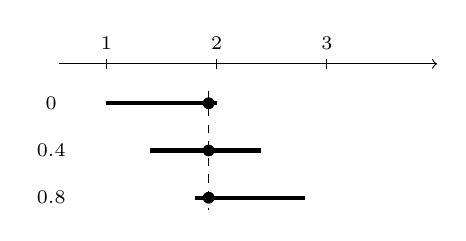
\begin{tikzpicture}[x=1mm,y=1mm,font=\scriptsize]

\draw[->] (14,22) -- (62,22);
\foreach \x/\lab in {20/1,34/2,48/3}
  \draw (\x,21.4) -- (\x,22.6) node[above=0pt]{\lab};

\node[] at (13,17) {$0$};
\draw[line width=1.5pt] (20,17) -- (34,17);

\myvdots{13}{14.7}{0.7}{0.1}

\node at (13,11) {$0.4$};
\draw[line width=1.5pt] (25.6,11) -- (39.6,11);

\myvdots{13}{8.7}{0.7}{0.1}

\node at (13,5) {$0.8$};
\draw[line width=1.5pt] (31.2,5) -- (45.2,5);

\myvdots{13}{2.7}{0.7}{0.1}

\draw[dashed] (33,18.5) -- (33,3.5);
\foreach \y in {17,11,5}
  \fill (33,\y) circle (0.75);

\end{tikzpicture}
\caption{$\kI=[1,2]$}\label{fig:non_punctual}
\end{subfigure}
\hfill
\begin{subfigure}[t]{0.47\textwidth}
\centering
\begin{tikzpicture}[x=1mm,y=1mm,font=\scriptsize]

\draw[->] (14,22) -- (62,22);
\foreach \x/\lab in {20/1,34/2,48/3}
  \draw (\x,21.4) -- (\x,22.6) node[above=0pt]{\lab};

\node at (13,17) {$0$};
\fill (20,17) circle (0.75);

\myvdots{13}{14.7}{0.7}{0.1}

\node at (13,11) {$0.4$};
\fill (25.6,11) circle (0.75);

\myvdots{13}{8.7}{0.7}{0.1}

\node at (13,5) {$0.8$};
\fill (31.2,5) circle (0.75);

\myvdots{13}{2.7}{0.7}{0.1}

\end{tikzpicture}
\caption{$\kI=[1,1]$}\label{fig:punctual}
\end{subfigure}

\caption{Onsets of a persistent demand and their windows.
% Non-singular windows of
%nearby onsets share a common time, so the pending obligations collapse to a single
%earliest deadline and one formula-clock $x_\mu$ records it; singular windows admit
%no such sharing.
}
\label{fig:punctual_vs_nonpunctual}
\end{figure}


The procedure is sound and terminating for all of TCTL. Completeness, however, is confined to
the non-punctual case, and rests on the single formula-clock: a persistent context re-demands
$\mu$ at a continuum of onsets, and one $x_\mu$ serves them all only because their windows
overlap. For $\kI=[a,b]$ with $a<b$, onsets near one another share a common time
(Fig.~\ref{fig:non_punctual}), so the pending obligations collapse to a single earliest deadline,
which is exactly what $x_\mu$ records. For $\kI=[a,a]$ (Fig.~\ref{fig:punctual}) the windows are pairwise disjoint
singletons, no witness serves two onsets, and the obligations a model carries at a given moment
depend on the exact offsets of every onset still pending. Such a model projects onto no finite
set of nodes, and the accepting lasso of Theorem~\ref{thm:completeness} need not exist. Therefore, on punctual intervals, although the tableau procedure still runs and terminates, it may fail to find a successful marking for a satisfiable formula. 

In practice, however, the full generality of TCTL is rarely needed. The most common use is
limited to properties of temporal nesting depth at most one, i.e.\ state reachability, safety and
inevitability, as supported by tools such as
\textsc{Uppaal}~\cite{BehrmannLarsenYi2004Uppaal} and \textsc{Romeo}~\cite{lime-TACAS-09} (the one exception being the leads-to query). There the continuum of onsets never arises: a modality whose argument is propositional is demanded once, at the configuration where \ruleref{Cov} fires,
and never re-imposed inside another pursuit. The obligations live at a node are then exactly the
pursuits it carries, all of them recorded in $\Gamma$, $\Ctx$ and $\Deadline$ with their elapsed time in
$Z$, so two nodes that agree componentwise agree on the obligation state itself, whatever the
intervals. We formalise this in the following corollary.

\begin{corollary}\label{cor:depthone}
The tableau procedure is sound and complete for TCTL of temporal nesting depth at most one.
\end{corollary}
\begin{proof}
Soundness follows from Theorem~\ref{thm:soundness}. The completeness argument of Theorem~\ref{thm:completeness} is unchanged up to the projection
step. Fresh onsets arise only when a modality is
demanded inside another's pursuit, which at depth one cannot happen, every argument being
propositional. A repeat $N_i\equiv N_j$ therefore agrees on the full obligation state, and the
projection goes through for every $\kI$.
\end{proof}

Leads-to queries, written $\mathrm{AG}(p\rightarrow\mathrm{AF}_\kI q)$, have depth two and
fall outside the corollary, as the outer modality re-demands the inner one at a continuum of onsets. They remain covered by
Theorem~\ref{thm:completeness} whenever $\kI$ is non-punctual.



%%%%%%%%%%%%%%%%%%%%%%%%%%%%%%%%%%%%%%%%%%%%%%%%%%%%%%%%%%%%%%%%%%%%%%%%%%%%%%




%
%\begin{remark}[Zeno semantics]
%Restricting to non-Zeno runs is the standard reading and the one our witnesses realise; the time-progress
%test~(ii), shown necessary and sufficient by Lemma~\ref{lem:nonzeno}, is what enforces it. We do not claim a
%free switch to the unrestricted semantics: admitting Zeno runs changes the meaning of {universal}
%time-bounded eventualities -- a time-convergent run may never reach a window, so $\mathrm{A}(\varphi\,
%\mathbf{U}_{[a,b]}\,\psi)$ can fail for reasons (ii) was designed to exclude -- and reconciling that needs more
%than dropping the divergence step. The non-Zeno reading is the one we adopt and prove.
%\end{remark}

%\medskip\noindent
%Together, Theorems~\ref{thm:complexity}, \ref{thm:soundness}, and \ref{thm:completeness} give a sound,
%complete, and terminating decision procedure for non-punctual TCTL satisfiability, optimal in \textsc{ExpTime}
%and returning a finite timed automaton on success. Its three mechanisms -- the AND--OR marking for branching,
%the time-progress condition for Zeno-freedom, and the region-faithful check for dense deadlines -- are largely
%independent and we expect them to transfer to related dense-time branching logics; we evaluate a prototype in
%Section~\ref{sec:eval}. Natural next steps are a fully optimised implementation (ours is a prototype), the
%extraction of minimal witnesses, and a study of the punctual boundary and of metric extensions.
